\let\negmedspace\undefined
\let\negthickspace\undefined
\documentclass[journal,12pt,onecolumn]{IEEEtran}
\usepackage{cite}
\usepackage{amsmath,amssymb,amsfonts,amsthm}
\usepackage{algorithmic}
\usepackage{tasks}
\settasks{label=\brak{\Alph*}, label-width=3ex, item-indent=0pt, column-sep=2em}
\usepackage{graphicx}
\graphicspath{{./figs/}}
\usepackage{textcomp}
\usepackage{xcolor}
\usepackage{txfonts}
\usepackage{listings}
\usepackage{enumitem}
\usepackage{mathtools}
\usepackage{gensymb}
\usepackage{comment}
\usepackage{caption}
\usepackage[breaklinks=true]{hyperref}
\usepackage{tkz-euclide} 
\usepackage{listings}
\usepackage{gvv}                                        
%\def\inputGnumericTable{}                                 
\usepackage[latin1]{inputenc}     
\usepackage{xparse}
\usepackage{color}                  
                           
\usepackage{array}                                            
\usepackage{longtable}                              
          
\usepackage{calc}                                             
\usepackage{multirow}
\usepackage{multicol}
\usepackage{hhline}                                           
\usepackage{ifthen}   
                                         
\usepackage{lscape}
\usepackage{tabularx}
\usepackage{array}
\usepackage{float}
\usepackage{mhchem}
\newtheorem{theorem}{Theorem}[section]
\newtheorem{problem}{Problem}
\newtheorem{proposition}{Proposition}[section]
\newtheorem{lemma}{Lemma}[section]
\newtheorem{corollary}[theorem]{Corollary}
\newtheorem{example}{Example}[section]
\newtheorem{definition}[problem]{Definition}
\newcommand{\BEQA}{\begin{eqnarray}}
\newcommand{\EEQA}{\end{eqnarray}}
\newcommand{\define}{\stackrel{\triangle}{=}}
\theoremstyle{remark}
\newtheorem{rem}{Remark}

\begin{document}
\title{
ASSIGNMENT 1: GATE 2025 \\
CY: CHEMISTRY}
\author{EE25BTECH11039 - Manupati Manideep}
\maketitle
\renewcommand{\thefigure}{\theenumi}
\renewcommand{\thetable}{\theenumi}
\begin{enumerate}
\section*{Q.1 - Q.5 carry one mark each}
\item Courage: Bravery :: Yearning :
    \begin{enumerate}
        \item Longing
        \item Yelling
        \item Yawning
        \item Glaring
    \end{enumerate}    
    \hfill{\brak{\text{GATE CY-2025}}}
  




\item We \rule{2cm}{0.15mm} tennis in the lawn when it suddenly started to rain.
    \begin{enumerate}
        \begin{multicols}{2}
        \item have been playing
        \item had been playing
        \item could be playing
        \item would have been playing
        \end{multicols}
    \end{enumerate}     
    \hfill{\brak{\text{GATE CY-2025}}}
    



\item A $4 \times 4$ digital image has pixel intensities \brak{U} as shown in the figure. The number of pixels with $U \leq 4$ is:
    \begin{figure}[H]
        \centering
        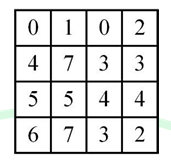
\includegraphics[width=0.2\columnwidth]{figs/q3.png}
        \caption*{}
        \label{fig:placeholder}
    \end{figure}
    \begin{enumerate}
        \begin{multicols}{4}
        \item 3
        \item 8
        \item 11
        \item 9
        \end{multicols}
    \end{enumerate}     
    \hfill{\brak{\text{GATE CY-2025}}}





\item In the given figure, the numbers associated with the rectangle, triangle, and ellipse are 1, 2, and 3, respectively. Which one among the given options is the most appropriate combination of P, Q, and R ?
    \begin{figure}[H]
        \centering
        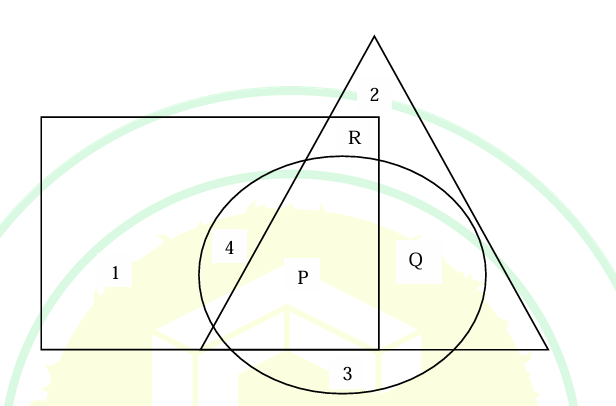
\includegraphics[width=0.4\columnwidth]{figs/q4.png}
        \caption*{}
        \label{fig:placeholder}
    \end{figure}
    \begin{enumerate}
        \item $P=6$; $Q=5$; $R=3$
        \item $P=5$; $Q=6$ $R=3$
        \item $P=3$; $Q=6$; $R=6$
        \item $P=5$ ; $Q=3$; $R=6$
    \end{enumerate}     
     \hfill{\brak{\text{GATE CY-2025}}}




\item A rectangle has a length L and a width W, where $L>W$ If the width, W, is increased by 10\%, which one of the following statements is correct for all values of L and W?
    \begin{enumerate}
        \item Perimeter increases by 10\%.
        \item Length of the diagonals increases by 10\%.
        \item Area increases by 10\%.
        \item The rectangle becomes a square.
    \end{enumerate}      \hfill{\brak{\text{GATE CY-2025}}}


\section*{Q.6 - Q.10 carry two marks each}
\item Column-I has statements made by Shanthala; and, Column-II has responses given by Kanishk. Identify the option that has the correct match between Column-I and Column-II.

\begin{itemize}
    \item P. This house is in a mess.
    \item Q. I am not happy with the marks given to me.
    \item R. Politics is a subject I avoid talking about.
    \item S. I don't know what this word means.
\end{itemize}

\begin{itemize}
    \item 1. Alright, I won't bring it up during our conversations.
    \item 2. Well, you can easily look it up.
    \item 3. No problem, let me clear it up for you.
    \item 4. Don't worry, I will take it up with your teacher.
\end{itemize}

    \begin{enumerate}
        \item P-2; Q-3; R-1; S-4
        \item P-3; Q-4; R-1; S-2
        \item P-4; Q-1; R-2; S-3
        \item P-1; Q-2; R-4; S-3
    \end{enumerate}      \hfill{\brak{\text{GATE CY-2025}}}



\item Weight of a person can be expressed as a function of their age. The function usually varies from person to person. Suppose this function is identical for two brothers, and it monotonically increases till the age of 50 years and then it monotonically decreases. Let $a_{1}$ and $a_{2}$ \brak{in years} denote the ages of the brothers and $a_{1}<a_{2}$. Which one of the following statements is correct about their age on the day when they attain the same weight?
    \begin{enumerate}
        \item $a_{1}<a_{2}<50$
        \item $a_{1}<50<a_{2}$
        \item $50<a_{1}<a_{2}$
        \item Either $a_{1}=50$ or $a_{2}=50$
    \end{enumerate}      \hfill{\brak{\text{GATE CY-2025}}}



\item A regular dodecagon \brak{\text{12-sided regular polygon}} is inscribed in a circle of radius r cm as shown in the figure. The side of the dodecagon is d cm. All the triangles \brak{\text{numbered 1 to 12}} in the figure are used to form squares of side r cm and each numbered triangle is used only once to form a square. The number of squares that can be formed and the number of triangles required to form each square, respectively, are:
    \begin{figure}[H]
        \centering
        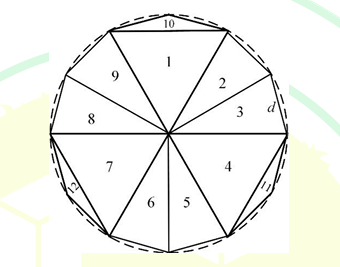
\includegraphics[width=0.4\columnwidth]{figs/q8.png}
        \caption*{}
        \label{fig:placeholder}
    \end{figure}
    \begin{enumerate}
        \item 3; 4
        \item 4; 3
        \item 3; 3
        \item 3; 2
    \end{enumerate}      \hfill{\brak{\text{GATE CY-2025}}}



\item If a real variable x satisfies $3^{x^{2}}=27\times9^{x}$ then the value of $\frac{2^{x^{2}}}{\brak{2^{x}}^{2}}$ is:
    \begin{enumerate}
        \begin{multicols}{2}
        \item $2^{-1}$
        \item $2^{0}$
        \item $2^{3}$
        \item 215
        \end{multicols}
    \end{enumerate}      \hfill{\brak{\text{GATE CY-2025}}}



\item The number of patients per shift \brak{X} consulting Dr. Gita in her past 100 shifts is shown in the figure. If the amount she earns is $\times1000\brak{X-0.2}$, what is the average amount \brak{in} she has earned per shift in the past 100 shifts?
    \begin{figure}[H]   
        \centering
        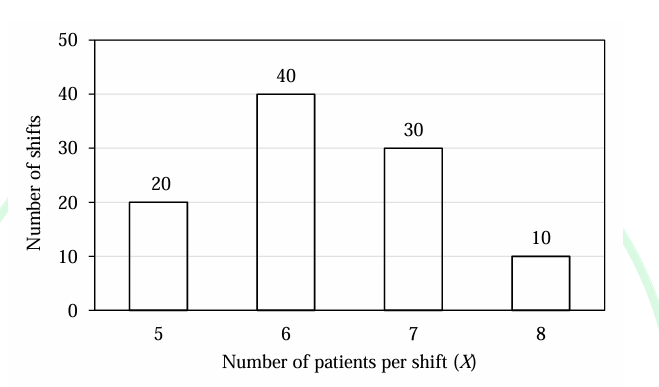
\includegraphics[width=0.4\columnwidth]{figs/q10.png}
        \caption*{}
        \label{fig:placeholder}
    \end{figure}
    \begin{enumerate}
        \begin{multicols}{2}
        \item 6,100
        \item 6,300
        \item 6,500
        \item 6,700
        \end{multicols}
    \end{enumerate}      \hfill{\brak{\text{GATE CY-2025}}}

\section*{Q.11 - Q.35 carry one mark each}    
  \item The phosphazene compound that acts as a superbase is
  \begin{multicols}{2}
      
    \begin{enumerate}
        \item 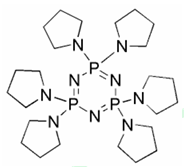
\includegraphics[width=0.3\columnwidth]{figs/q11a.png}
        \item 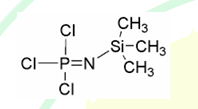
\includegraphics[width=0.3\columnwidth]{figs/q11b.png}
        \item 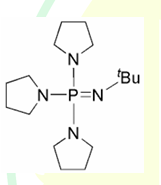
\includegraphics[width=0.3\columnwidth]{figs/q11c.png}
        \item 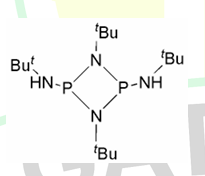
\includegraphics[width=0.3\columnwidth]{figs/q11d.png}
    \end{enumerate}      \hfill{\brak{\text{GATE CY-2025}}}
    \end{multicols}



\item The reaction for the synthesis of Me$_{2}$SiCl$_{2}$ through Rochow-Müller process is
    \begin{enumerate}
        \item 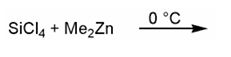
\includegraphics[width=0.3\columnwidth]{figs/q12a.png}
        \item 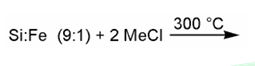
\includegraphics[width=0.3\columnwidth]{figs/q12b.png}
        \item 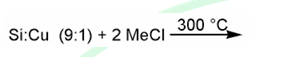
\includegraphics[width=0.3\columnwidth]{figs/q12c.png}
        \item 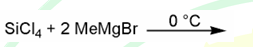
\includegraphics[width=0.3\columnwidth]{figs/q12d.png}
    \end{enumerate}      \hfill{\brak{\text{GATE CY-2025}}}



\item Upon cooling from room temperature, the magnetic susceptibility of MnO slowly increases until 118 K, and then it decreases. This phenomenon is known as
    \begin{enumerate}
        \item ferromagnetism
        \item paramagnetism
        \item antiferromagnetism
        \item ferrimagnetism
    \end{enumerate}      \hfill{\brak{\text{GATE CY-2025}}}



\item An aqueous solution of Co\brak{ClO_{4}}$_{2}$$\cdot$6H$_{2}$O is light pink in colour. Addition of conc. HCl results in an intense blue coloured solution due to the formation of a new species. The new species among the following is
 \begin{figure}[H]
        \centering
        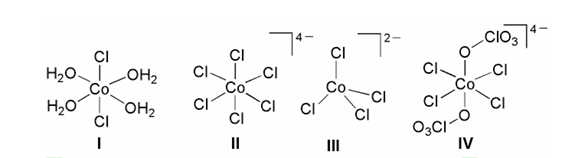
\includegraphics[width=0.4\columnwidth]{figs/q14.png}
        \caption*{}
        \label{fig:placeholder}
    \end{figure}
    \begin{multicols}{4}
        
    \begin{enumerate}
    \item 1
    \item 2
    \item 3
    \item 4
    \end{enumerate}      \hfill{\brak{\text{GATE CY-2025}}}
    \end{multicols}



\item For an unambiguous single step synthesis of the following target molecule \brak{TM}, the best bond disconnection in its retrosynthetic analysis is
 \begin{figure}[H]
        \centering
        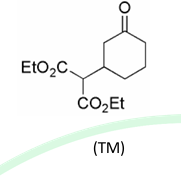
\includegraphics[width=0.4\columnwidth]{figs/q15.png}
        \caption*{}
        \label{fig:placeholder}
    \end{figure}
     \begin{multicols}{2}
    \begin{enumerate}
        \item 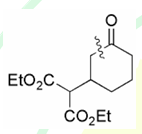
\includegraphics[width=0.2\columnwidth]{figs/q15a.png}
        \item 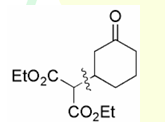
\includegraphics[width=0.2\columnwidth]{figs/q15b.png}
        \item 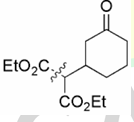
\includegraphics[width=0.2\columnwidth]{figs/q15c.png}
        \item 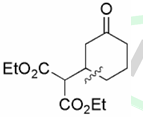
\includegraphics[width=0.2\columnwidth]{figs/q15d.png}
    \end{enumerate}      \hfill{\brak{\text{GATE CY-2025}}}
    \end{multicols}



\item In the $^{1}$H-NMR spectrum of the following molecule, the signal of proton H$_{a}$ appears as
 \begin{figure}[H]
        \centering
        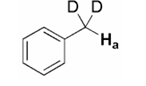
\includegraphics[width=0.4\columnwidth]{figs/q16.png}
        \caption*{}
        \label{fig:placeholder}
    \end{figure}
    \begin{enumerate}
        \item singlet
        \item triplet
        \item quintet
        \item quartet
    \end{enumerate}      \hfill{\brak{\text{GATE CY-2025}}}



\item A disaccharide X does NOT show mutarotation in aqueous solution. Acidic hydrolysis of X affords two different monosaccharides. The disaccharide X is
 \begin{multicols}{2}
    \begin{enumerate}
        \item 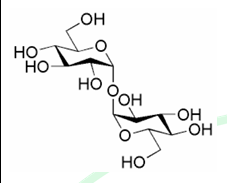
\includegraphics[width=0.25\columnwidth]{figs/q17a.png}
        \item 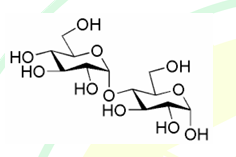
\includegraphics[width=0.25\columnwidth]{figs/q17b.png}
        \item 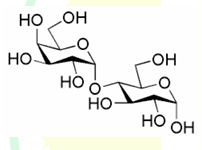
\includegraphics[width=0.25\columnwidth]{figs/q17c.png}
        \item 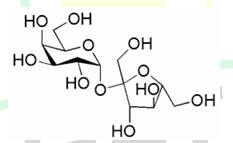
\includegraphics[width=0.25\columnwidth]{figs/q17d.png}
    \end{enumerate}      \hfill{\brak{\text{GATE CY-2025}}}
    \end{multicols}



\item The symmetry element that does NOT belong to $C_{4v}$ point group is
    \begin{enumerate}
        \item $C_{4}$
        \item $C_{2}$
        \item $i$
        \item $\sigma_{v}$
    \end{enumerate}      \hfill{\brak{\text{GATE CY-2025}}}



\item Rigid rotor wavefunctions are given by $Y_{l,m}\brak{\theta,\phi}$. The wavefunctions $Y_{1,0}\brak{\theta, \phi}$ and $Y_{2,0}\brak{\theta,\phi}$ are given below
    \begin{center}
        $Y_{1,0}\brak{\theta, \phi} = \sqrt{\frac{3}{4\pi}}cos \theta$
       
        $Y_{2,0}\brak{\theta,\phi} = \sqrt{\frac{5}{16\pi}}\brak{3 cos^{2}\theta - 1}$
    \end{center}
    For a non-polar diatomic molecule, the value of transition dipole moment integral for transition between $Y_{1,0}\brak{\theta, \phi}$ and $Y_{2,0}\brak{\theta,\phi}$ is equal to
    \begin{enumerate}
        \item $\frac{1}{\sqrt{2\pi}}$
        \item 0
        \item 2
        \item $\frac{1}{\sqrt{4\pi}}$
    \end{enumerate}      \hfill{\brak{\text{GATE CY-2025}}}



\item The translational, vibrational, and rotational molecular partition functions for a system containing ideal diatomic gas molecules in the canonical ensemble \brak{N, V, T} are written as, $q_{trans}$, $q_{vib}$, and $q_{rot}$, respectively. The option that correctly defines their thermodynamic variable\brak{s} dependency is
    \begin{enumerate}
        \item $q_{trans} \brak{T, V}, q_{vib} \brak{T, V}, q_{rot}\brak{T, V}$
        \item $q_{trans} \brak{T, V}, q_{vib} \brak{T}, q_{rot}\brak{T}$
        \item $q_{trans} \brak{T}, q_{vib} \brak{T, V}, q_{rot}\brak{T}$
        \item $q_{trans} \brak{T, V}, q_{vib} \brak{T}, q_{rot}\brak{T, V}$
    \end{enumerate}      \hfill{\brak{\text{GATE CY-2025}}}
\item The Vaska's complex trans-IrCl\brak{CO}\brak{PPh_{3}}$_{2}$ shows a band at 1967 cm$^{-1}$ for the $\nu_{CO}$ stretching vibration in its infrared spectrum. The complexes that will show an increase in the $\nu_{CO}$ stretching vibration from 1967 cm$^{-1}$ is/are
 \begin{multicols}{2}
    \begin{enumerate}
        \item 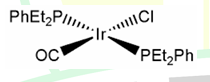
\includegraphics[width=0.2\columnwidth]{figs/q21a.png}
        \item 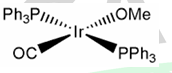
\includegraphics[width=0.2\columnwidth]{figs/q21b.png}
        \item 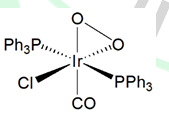
\includegraphics[width=0.2\columnwidth]{figs/q21c.png}
        \item 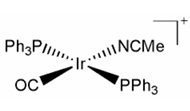
\includegraphics[width=0.2\columnwidth]{figs/q21d.png}
    \end{enumerate}      \hfill{\brak{\text{GATE CY-2025}}}
    \end{multicols}



\item Under the conditions mentioned for each reaction, the reaction\brak{s} that would give borazine \brak{B_{3}N_{3}H_{6}} as the major product is/are
    \begin{enumerate}
        \item 3 BCl$_{3}$ + 3 NH$_{4}$Cl $\xrightarrow{140^{\circ}C}$
        \item B$_{2}$H$_{6}$ + 2 NH$_{3}$ $\xrightarrow{>250^{\circ}C}$
        \item 3 B$_{2}$H$_{6}$ + 6 NH$_{4}$Cl $\xrightarrow{\text{ether solvent}}$
        \item 3 LiBH$_{4}$ + 3 NH$_{4}$Cl $\xrightarrow{\text{THF reflux}}$
    \end{enumerate}      \hfill{\brak{\text{GATE CY-2025}}}



\item The essential symmetries for a monoclinic crystal system is/are the presence of
    \begin{enumerate}
        \item one C$_{3}$ axis
        \item one C$_{2}$ axis
        \item one C$_{4}$ axis
        \item one C$_{6}$ axis
    \end{enumerate}      \hfill{\brak{\text{GATE CY-2025}}}



\item Compound\brak{s} that show\brak{s} an intense peak at m/z 120 in the EI mass spectrum is/are
    \begin{enumerate}
        \item 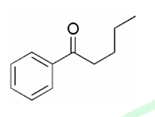
\includegraphics[width=0.2\columnwidth]{figs/q24a.png}
        \item 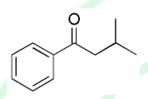
\includegraphics[width=0.2\columnwidth]{figs/q24b.png}
        \item 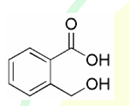
\includegraphics[width=0.2\columnwidth]{figs/q24c.png}
        \item 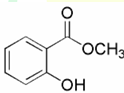
\includegraphics[width=0.2\columnwidth]{figs/q24d.png}
    \end{enumerate}      \hfill{\brak{\text{GATE CY-2025}}}



\item The correct option\brak{s} of reagents and reaction sequences suitable for carrying out the following transformation is/are
    \begin{enumerate}
        \item \brak{i} NBS, \brak{PhCOO}$_{2}$; \brak{ii} aq. NaOH; \brak{iii} active MnO$_{2}$; \brak{iv} Li/liq.NH$_{3}$, t-BuOH
        \item \brak{i} m-CPBA; \brak{ii} BF$_{3}$.Et$_{2}$O
        \item \brak{i} SeO$_{2}$; \brak{ii} Dess-Martin periodinane; \brak{iii} K\sbrak{BH\brak{s-Bu}_{3}} \brak{K-selectride}
        \item \brak{i} dil. KMnO$_{4}$; \brak{ii} NaIO$_{4}$
    \end{enumerate}      \hfill{\brak{\text{GATE CY-2025}}}



\item Among the given options, the possible product\brak{s} that can be obtained from the following reaction is/are
 \begin{figure}[H]
        \centering
        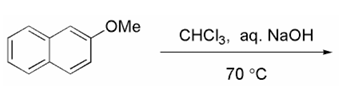
\includegraphics[width=0.4\columnwidth]{figs/q26.png}
        \caption*{}
        \label{fig:placeholder}
    \end{figure}
     \begin{multicols}{2}
    \begin{enumerate}
        \item 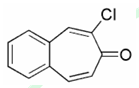
\includegraphics[width=0.2\columnwidth]{figs/q26a.png}
        \item 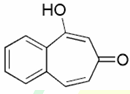
\includegraphics[width=0.2\columnwidth]{figs/q26b.png}
        \item 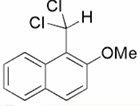
\includegraphics[width=0.2\columnwidth]{figs/q26c.png}
        \item 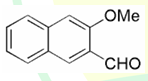
\includegraphics[width=0.2\columnwidth]{figs/q26d.png}
    \end{enumerate}      \hfill{\brak{\text{GATE CY-2025}}}
    \end{multicols}



\item Choose the correct option\brak{s} with regard to mechanism of the following transformation.
    \begin{enumerate}
        \item It proceeds through divinyl cyclopropane rearrangement
        \item It involves a diradical intermediate
        \item It proceeds through di-$\pi$-methane rearrangement
        \item It proceeds through [2+2+2] cycloaddition reaction
    \end{enumerate}      \hfill{\brak{\text{GATE CY-2025}}}



\item Consider two non-interacting particles confined to a one-dimensional box with infinite potential barriers. Their wavefunctions are $\psi_{1}$ and $\psi_{2}$ and energies are E$_{1}$ and E$_{2}$, respectively. The INCORRECT statement\brak{s} about this system is/are
    \begin{enumerate}
        \item The total energy is E$_{1}$ + E$_{2}$
        \item The total wavefunction is $\psi_{1}$ + $\psi_{2}$
        \item The total energy is E$_{1}$E$_{2}$
        \item The total wavefunction is $\psi_{1}\psi_{2}$
    \end{enumerate}      \hfill{\brak{\text{GATE CY-2025}}}



\item The thermodynamic criterion/criteria for a spontaneous process is/are
    \begin{enumerate}
        \item $\Delta$U $>$ 0 at constant S and V
        \item $\Delta$S $>$ 0 at constant U and V
        \item $\Delta$\brak{H - TS} $>$ 0 at constant T and P
        \item $\Delta$\brak{U - TS} $<$ 0 at constant T and V
    \end{enumerate}      \hfill{\brak{\text{GATE CY-2025}}}



\item Xe and F$_{2}$ in 1:1 molar ratio when mixed in a closed flask and kept in the sunlight for a day, gave white crystals of a compound Q. Two equivalents of Q on reaction with one equivalent of AsF$_{5}$ gave an ionic compound X + Y with the cation having two Xe atoms. The total number of lone pairs present on the cation X$^{+}$ is \_\_\_\_ \brak{\text{in integer}}. \hfill{\brak{\text{GATE CY-2025}}}


\item The total number of hyperfine lines expected in the EPR spectrum of CH$_{2}$OH \brak{radical} is \_\_\_\_ \brak{\text{in integer}}. \hfill{\brak{\text{GATE CY-2025}}}
\sbrak{Note: Consider all hydrogen atoms for calculation}




\item Partial hydrolysis of a pentapeptide yields all possible tripeptides and dipeptides. The dipeptides that are obtained upon hydrolysis are given below.

Val-Ala, Gln-His, Phe-Val and Ala-Gln
 \hfill{\brak{\text{GATE CY-2025}}}

The total number of tripeptides obtained that contain 'Ala' as one of the amino acids is\_\_\_\_ \brak{\text{in integer}} \hfill{\brak{\text{GATE CY-2025}}}





\item The specific rotation of enantiomerically pure \brak{S}-2-butanol is +14$^{\circ}$. The specific rotation of enantiomeric mixture of 2-butanol obtained from an asymmetric reduction of 2-butanone is found to be +7$^{\circ}$. The percentage of \brak{R}-2-butanol present in the reaction mixture is \_\_\_\_ \brak{\text{in integer}}. \hfill{\brak{\text{GATE CY-2025}}}





\item The ratio of the fundamental vibrational frequencies $\brak{\frac{\nu_{^{13}C^{16}O}}{\nu_{^{12}C^{16}O}}}$ of two diatomic molecules $^{13}$C$^{16}$O and $^{12}$C$^{16}$O, considering their force constants to be the same, is \_\_\_\_\_ \brak{\text{rounded off to two decimal places}} \hfill{\brak{\text{GATE CY-2025}}}




\item The expressions for the vapour pressure of solid \brak{p_1} and vapour pressure of liquid \brak{p_2} phases of a pure substance, respectively, are

$\ln p_1 = -\frac{2000}{T}+ 5$ and $\ln p_2 = -\frac{4000}{T}+ 10$

The triple point temperature of this substance is \_\_\_\_ K \brak{\text{in integer}}. \hfill{\brak{\text{GATE CY-2025}}}



\section*{Q.36 - Q.65 carry two marks each}

\item The reaction that proceeds through an oxidative addition followed by a reductive elimination is

    \sbrak{given: Atomic numbers Ni = 28, Ta = 73, Zr = 40, Pt = 78}
    \begin{enumerate}
    
        \item 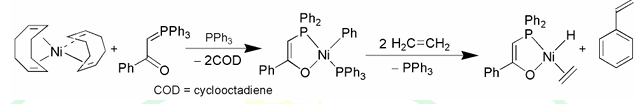
\includegraphics[width=0.6\columnwidth]{figs/q36a.png}
        \item 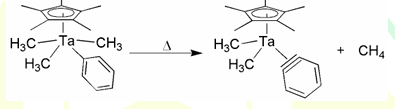
\includegraphics[width=0.6\columnwidth]{figs/q36b.png}
        \item 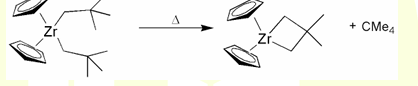
\includegraphics[width=0.6\columnwidth]{figs/q36c.png}
        \item 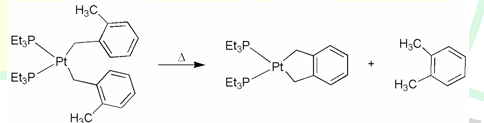
\includegraphics[width=0.6\columnwidth]{figs/q36d.png}
 
    \end{enumerate}      \hfill{\brak{\text{GATE CY-2025}}}



\item The homogeneous catalyst whose metal ion does NOT undergo either oxidation or reduction in any of the steps during the hydrogenation of terminal olefins is
    \begin{enumerate}
    \begin{multicols}{2}
        \item RhCl\brak{PPh_{3}}$_{3}$
        \item HRuCl\brak{PPh_{3}}$_{3}$
        \item [Ir\brak{COD}\brak{PCy_{3}}\brak{Py}]$^{+}$ PF$_{6}^{-}$ \brak{COD = cyclooctadiene}
        \item [Rh\brak{COD}\brak{PPh_{3}}$_{2}$]$^{+}$ PF$_{6}^{-}$ \brak{COD = cyclooctadiene}
    \end{multicols}
    \end{enumerate}      \hfill{\brak{\text{GATE CY-2025}}}



\item The given zirconocene compound, \brak{\eta^{5}-Cp}$_{2}$ZrEt$_{2}$, when heated in the presence of an equimolar amount of PMe$_{3}$ results in the formation of a compound X which obeys the 18 electron rule. The reaction also resulted in the release of a saturated hydrocarbon.

\sbrak{given: Atomic number of Zr = 40}

The structure of compound X is
 \begin{figure}[H]
        \centering
        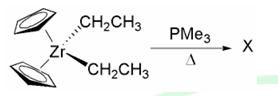
\includegraphics[width=0.4\columnwidth]{figs/q38.png}
        \caption*{}
        \label{fig:placeholder}
    \end{figure}
    \begin{enumerate}
    \begin{multicols}{2}
        \item 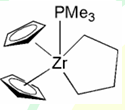
\includegraphics[width=0.3\columnwidth]{figs/q38a.png}
        \item 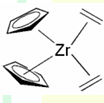
\includegraphics[width=0.3\columnwidth]{figs/q38b.png}
        \item 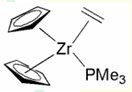
\includegraphics[width=0.3\columnwidth]{figs/q38c.png}
        \item 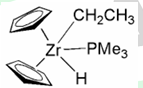
\includegraphics[width=0.3\columnwidth]{figs/q38d.png}
    \end{multicols}
    \end{enumerate}      \hfill{\brak{\text{GATE CY-2025}}}



\item The $^{1}$H NMR spectrum of the given iridium complex at room temperature gave a single signal at 2.6 ppm, and its $^{31}$P NMR spectrum gave a single signal at 23.0 ppm. When the spectra were recorded at lower temperatures, both these signals split into a complex pattern. The intra-molecular dynamic processes shown by this molecule are
    \begin{enumerate}
        \item Berry pseudo-rotation and rotation of the ethylene units along the C=C axis
        \item Berry pseudo-rotation and propeller type rotation of the ethylene units along the Ir-alkene axis
        \item Ray-Dutt twist and rotation of the ethylene units along the C=C axis
        \item Ray-Dutt twist and propeller type rotation of the ethylene units along the Ir-alkene axis
    \end{enumerate}      \hfill{\brak{\text{GATE CY-2025}}}



\item The effective magnetic moment, $\mu_{eff}$ value for [Cr\brak{H_{2}O}$_{6}$]$^{3+}$ taking into account for spin-orbit coupling is closest to

\sbrak{given: Atomic number of Cr = 24, spin-orbit coupling constant \lambda = 92 cm^{-1}, and \Delta_{o} = 17400 cm^{-1}}
    \begin{enumerate}
    \begin{multicols}{2}
        \item 3.79 $\mu_{B}$
        \item 3.87 $\mu_{B}$
        \item 4.05 $\mu_{B}$
        \item 3.60 $\mu_{B}$
    \end{multicols}
    \end{enumerate}      \hfill{\brak{\text{GATE CY-2025}}}

\item The major products X and Y formed in the following reaction sequences are
    \begin{figure}[H]
        \centering
        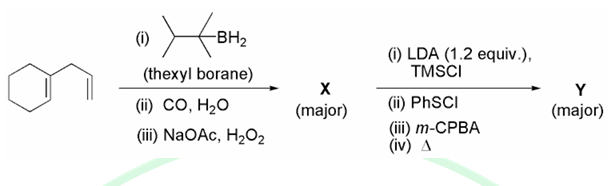
\includegraphics[width=0.4\columnwidth]{figs/q41.png}
        \caption*{}
        \label{fig:placeholder}
    \end{figure}
    \begin{enumerate}
        \item 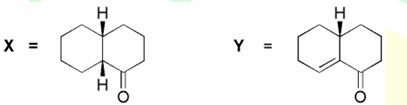
\includegraphics[width=0.6\columnwidth]{figs/q41a.png}
        \item 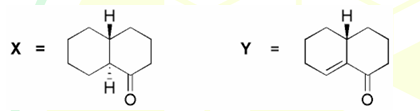
\includegraphics[width=0.6\columnwidth]{figs/q41b.png}
        \item 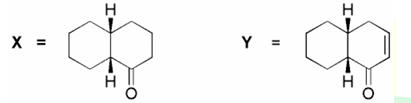
\includegraphics[width=0.6\columnwidth]{figs/q41c.png}
        \item 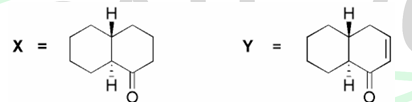
\includegraphics[width=0.6\columnwidth]{figs/q41d.png}
    \end{enumerate}      \hfill{\brak{\text{GATE CY-2025}}}



\item Compound K displayed a strong band at 1680 cm$^{-1}$ in its IR spectrum. Its $^{1}$H-NMR spectral data are as follows: $\delta$ \brak{ppm} 7.30 \brak{d, J = 7.2 Hz, 2H}, 6.8 \brak{d, J = 7.2 Hz, 2H}, 3.8 \brak{septet, J = 7.0 Hz, 1H}, 2.2 \brak{s, 3H}, 1.9 \brak{d, J = 7.0 Hz, 6H}. The correct structure of compound K is
 \begin{multicols}{2}
    \begin{enumerate}
        \item \includegraphics[width=0.25\columnwidth]{figs/q42a.png}
        \item \includegraphics[width=0.25\columnwidth]{figs/q42b.png}
        \item \includegraphics[width=0.25\columnwidth]{figs/q42c.png}
        \item \includegraphics[width=0.25\columnwidth]{figs/q42d.png}
    \end{enumerate}      \hfill{\brak{\text{GATE CY-2025}}}
    \end{multicols}



\item The major product formed in the following reaction sequences is
 \begin{figure}[H]
        \centering
        \includegraphics[width=0.4\columnwidth]{figs/q43.png}
        \caption*{}
        \label{fig:placeholder}
        \end{figure}
         \begin{multicols}{2}
    \begin{enumerate}
        \item \includegraphics[width=0.25\columnwidth]{figs/q43a.png}
        \item \includegraphics[width=0.25\columnwidth]{figs/q43b.png}
        \item \includegraphics[width=0.25\columnwidth]{figs/q43c.png}
        \item \includegraphics[width=0.25\columnwidth]{figs/q43d.png}
    \end{enumerate}      \hfill{\brak{\text{GATE CY-2025}}}
    \end{multicols}



\item In the following asymmetric transformation, the key aldol reaction involves the attack of
    \begin{enumerate}
        \item Si face of enolate on to the Re face of aldehyde
        \item Si face of enolate on to the Si face of aldehyde
        \item Re face of enolate on to the Re face of aldehyde
        \item Re face of enolate on to the Si face of aldehyde
    \end{enumerate}      \hfill{\brak{\text{GATE CY-2025}}}



\item The correct option with regard to the following statements is
    \begin{enumerate}
        \item \brak{a} Time-independent Schrödinger equation can be exactly solved for Be$^{2+}$.
        \item \brak{b} For a particle confined in a one-dimensional box of length $l$ with infinite potential barriers, the trial variation function $\phi = [\frac{3}{l^{3}}]^{1/2}x$ is not an acceptable trial wavefunction for $0 \le x \le l$.
        \item \brak{c} Wavefunctions for system of Fermions must be anti-symmetric with respect to exchange of any two Fermions in the system.
        \item \brak{d} Born-Oppenheimer approximation can be used to separate the vibrational and rotational motion of a molecule.
    \end{enumerate}      \hfill{\brak{\text{GATE CY-2025}}}



\item The phase diagram of a single component system is given below. The option with the correct number of degrees of freedom corresponding to the labelled points i, j, and k, respectively, is
\begin{figure}[H]
        \centering
        \includegraphics[width=0.4\columnwidth]{figs/q46.png}
        \caption*{}
        \label{fig:placeholder}
    \end{figure}
    \begin{enumerate}
        \item 0, 1, 2
        \item 3, 2, 1
        \item 2, 0, 1
        \item 0, 2, 1
    \end{enumerate}      \hfill{\brak{\text{GATE CY-2025}}}



\item An approximate partition function $Q\brak{N, V, T}$ of a gas is given below. $Q\brak{N, V, T} = \frac{1}{N!}\brak{\frac{2\pi mk_{B}T}{h^{2}}}^{3N/2}\brak{V - Nb}^{N}$ The equation of state\brak{s} for this gas is/are [Note: $b$ is a parameter independent of volume.]
    \begin{enumerate}
        \item $P\brak{V - Nb} = Nk_{B}T$
        \item $PV^{\brak{N-b}} = k_{B}T$
        \item $PV = Nk_{B}T$
        \item $P\brak{V - Nb} = Nk_{B}$
    \end{enumerate}      \hfill{\brak{\text{GATE CY-2025}}}



\item The compound\brak{s} having structure similar to that of B$_{2}$H$_{6}$ is/are
    \begin{enumerate}
        \item I$_{2}$Cl$_{6}$
        \item Si$_{2}$Cl$_{6}$
        \item Al$_{2}$Cl$_{6}$
        \item Cl$_{2}$O$_{6}$
    \end{enumerate}      \hfill{\brak{\text{GATE CY-2025}}}



\item The UV-visible spectrum of [Ni\brak{en}$_{3}$]$^{2+}$ \brak{\text{en = ethylenediamine}} shows absorbance maxima at 11200 cm$^{-1}$, 18350 cm$^{-1}$, and 29000 cm$^{-1}$. Absorbance maximum Electronic transition \brak{a} 11200 cm$^{-1}$ \brak{i} $^{3}$A$_{2g}$$\to$ $^{3}$T$_{1g}$ \brak{F} \brak{b} 18350 cm$^{-1}$ \brak{ii} $^{3}$A$_{2g}$$\to$ $^{3}$T$_{2g}$ \brak{c} 29000 cm$^{-1}$ \brak{iii} $^{3}$A$_{2g}$$\to$ $^{3}$T$_{1g}$ \brak{P} \sbrak{given: Atomic number of Ni = 28} The correct match\brak{es} between absorbance maximum and electronic transition is/are
    \begin{enumerate}
        \item \brak{a} $\to$ \brak{ii}
        \item \brak{b} $\to$ \brak{i}
        \item \brak{a} $\to$ \brak{iii}
        \item \brak{c} $\to$ \brak{iii}
    \end{enumerate}      \hfill{\brak{\text{GATE CY-2025}}}



\item Cytochrome P450 \brak{CYP} enzymes catalyze stereoselective C$\text{--}$H hydroxylation of hydrocarbons in the presence of O$_{2}$. The correct statement\brak{s} about the structure and activity of CYP is/are
    \begin{enumerate}
        \item A thiolate group is coordinated to the Fe center at one of the axial positions around Fe.
        \item While one of the oxygen atoms of O$_{2}$ is inserted into a C$\text{--}$H bond of a hydrocarbon, the other oxygen atom gets reduced to water.
        \item An imidazole group is coordinated to the Fe center at one of the axial positions around Fe.
        \item An iron-oxo species acts as a key oxidant in the catalytic cycle of CYP.
    \end{enumerate}      \hfill{\brak{\text{GATE CY-2025}}}
    \item The complex\brak{es} having metal-metal bond order $\ge$3.5 is/are

\sbrak{given: The atomic numbers of Mo, Cr, Mn, and Re are 42, 24, 25, and 75, respectively.}
    \begin{enumerate}
     \item $[Ti\brak{H_2O}_6]^{3+}$ $<$ $[Mn\brak{H_2O}_6]^{2+}$ $<$ $[CrO_4]^{2-}$
    \item $[Mn\brak{H_2O}_6]^{2+}$ $<$ $[Ti\brak{H_2O}_6]^{3+}$ $<$ $[CrO_4]^{2-}$
    \item $[NiCl_4]^{2-}$ $<$ $[Ti\brak{H_2O}_6]^{3+}$ $<$ $[Mn\brak{H_2O}_6]^{2+}$
    \item $[NiCl_4]^{2-}$ $<$ $[Mn\brak{H_2O}_6]^{2+}$ $<$ $[Ti\brak{H_2O}_6]^{3+}$
    
    \end{enumerate}      \hfill{\brak{\text{GATE CY-2025}}}



\item Consider the following two reactions and their corresponding Hammett plots

Choose the option\brak{s} that correctly match\brak{es} the points on the graph given in Column-I with substituents X given in Column-II in accordance with their substituents constant $\sigma$

Column-I \brak{\text{points on the graph}} \quad Column-II \brak{\text{substituent X}}

p \quad NH$_{2}$

q \quad NO$_{2}$

r \quad OMe

s \quad Cl

t \quad Me

u \quad CN
    \begin{enumerate}
    \begin{multicols}{2}
        \item s $\to$ $\sigma$\brak{X = Cl}; t $\to$ $\sigma$\brak{X = OMe}; u $\to$ $\sigma$\brak{X = NH_{2}}; r $\to$ $\sigma$\brak{X = NO_{2}}
        \item s $\to$ $\sigma$\brak{X = Me}; u $\to$ $\sigma$\brak{X = NH_{2}}; t $\to$ $\sigma$\brak{X = OMe}; r $\to$ $\sigma$\brak{X = Br}
        \item p $\to$ $\sigma$\brak{X = Me}; q $\to$ $\sigma$\brak{X = CN}; r $\to$ $\sigma$\brak{X = NO_{2}}; t $\to$ $\sigma$\brak{X = OMe}
        \item p $\to$ $\sigma$\brak{X = Cl}; q $\to$ $\sigma$\brak{X = NO_{2}}; r $\to$ $\sigma$\brak{X = CN}; t $\to$ $\sigma$\brak{X = Me}
    \end{multicols}
    \end{enumerate}      \hfill{\brak{\text{GATE CY-2025}}}



\item The correct option\brak{s} of reagents and reaction sequences suitable for carrying out the following transformation is/are
 \begin{figure}[H]   
        \centering
        \includegraphics[width=0.4\columnwidth]{figs/q53.png}
        \caption*{}
        \label{fig:placeholder}
    \end{figure}
    \begin{enumerate}
  
        \item \includegraphics[width=0.6\columnwidth]{figs/q53a.png}
        \item \includegraphics[width=0.6\columnwidth]{figs/q53b.png}
        \item \includegraphics[width=0.6\columnwidth]{figs/q53c.png}
        \item \includegraphics[width=0.6\columnwidth]{figs/q53d.png}
   
    \end{enumerate}      \hfill{\brak{\text{GATE CY-2025}}}



\item The process\brak{es} and/or intermediate\brak{s} through which the following transformation proceeds is/are
 \begin{figure}[H]   
        \centering
        \includegraphics[width=0.4\columnwidth]{figs/q54.png}
        \caption*{}
        \label{fig:placeholder}
    \end{figure}
    \begin{enumerate}
    \begin{multicols}{2}
        \item 1,2-methide shift
        \item 1,3-methide shift
        \item non-classical carbocation
        \item tertiary carbocation
    \end{multicols}
    \end{enumerate}      \hfill{\brak{\text{GATE CY-2025}}}



\item For the following reaction, the possible product\brak{s} is/are
    \begin{enumerate}
    \begin{multicols}{2}
        \item \includegraphics[width=0.4\columnwidth]{figs/q55a.png}
        \item \includegraphics[width=0.4\columnwidth]{figs/q55b.png}
        \item \includegraphics[width=0.4\columnwidth]{figs/q55c.png}
        \item \includegraphics[width=0.4\columnwidth]{figs/q55d.png}
    \end{multicols}
    \end{enumerate}      \hfill{\brak{\text{GATE CY-2025}}}



\item Wavefunctions and energies for a particle confined in a cubic box are $\psi_{n_x, n_y, n_z}$ and $E_{n_x, n_y, n_z}$, respectively. The functions $\phi_1$, $\phi_2$, $\phi_3$, and $\phi_4$ are written as linear combinations of $\psi_{n_x, n_y, n_z}$. Among these functions, the eigenfunction\brak{s} of the Hamiltonian operator for this particle is/are

$\phi_1 = \frac{1}{\sqrt{2}}\psi_{1,4,1} - \frac{1}{\sqrt{2}}\psi_{2,2,3}$

$\phi_2 = \frac{1}{\sqrt{2}}\psi_{1,5,1} + \frac{1}{\sqrt{2}}\psi_{3,3,3}$

$\phi_3 = \frac{1}{\sqrt{2}}\psi_{1,3,8} + \frac{1}{\sqrt{2}}\psi_{3,8,1}$

$\phi_4 = \frac{1}{2}\psi_{3,3,1} + \frac{\sqrt{3}}{2}\psi_{2,4,1}$
    \begin{enumerate}
    \begin{multicols}{2}
        \item $\phi_2$
        \item $\phi_4$
        \item $\phi_3$
        \item $\phi_1$
    \end{multicols}
    \end{enumerate}      \hfill{\brak{\text{GATE CY-2025}}}



\item If a particle's state function is an eigenfunction of the operator $\hat{L}^2$ with eigenvalue $30\hbar^2$, then the possible eigenvalue\brak{s} of the operator $\hat{L}_z^2$ for the same state function is/are
    \begin{enumerate}
    \begin{multicols}{2}
        \item 10$\hbar^2$
        \item 16$\hbar^2$
        \item 25$\hbar^2$
        \item 0
    \end{multicols}
    \end{enumerate}      \hfill{\brak{\text{GATE CY-2025}}}



\item An archaeological specimen containing $^{14}$C gives 45 counts per gram of carbon in 5 minutes. A specimen of freshly cut wood gives 20 counts per gram of carbon per minute. The counter used recorded a background count of 5 counts per minute in the absence of any $^{14}$C containing sample. The age of the specimen is \_\_\_\_ years \brak{\text{in integer}}. [Note: $t_{1/2}$ of $^{14}$C = 5730 years]
 \hfill{\brak{\text{GATE CY-2025}}}





\item In the following reaction, 13.4 grams of aldehyde P gave a diastereomeric mixture of alcohols Q and R in a ratio of 2:1. If the yield of the reaction is 80, then the amount of Q \brak{in grams} obtained is \_\_\_\_ \brak{\text{in integer}}. \hfill{\brak{\text{GATE CY-2025}}}





\item The kinetic energies of an electron \brak{e} and a proton \brak{p} are $E$ and $3E$, respectively. Given that mass of a proton is 1836 times that of an electron, the ratio of their de Broglie wavelengths \brak{\frac{\lambda_e}{\lambda_p}} is \_\_\_\_ \brak{\text{rounded off to two decimal places}}. \hfill{\brak{\text{GATE CY-2025}}}


\item If a molecule emitting a radiation of frequency 3.100 $\times$ 10$^{9}$ Hz approaches an observer with a relative speed of 5.000 $\times$ 10$^{6}$ m s$^{-1}$, then the observer detects a frequency of \_\_\_\_ $\times$ 10$^{9}$ Hz \brak{\text{rounded off to three decimal places}}
 \hfill{\brak{\text{GATE CY-2025}}}


\sbrak{given: Speed of light c = 3.000 \times 10^{8} m s^{-1}}



\item The mean energy of a molecule having two available energy states at $\epsilon$ = 0 J and $\epsilon$ = 4.14 $\times$ 10$^{-21}$ J at 300 K is \_\_\_\_$\times$ 10$^{-21}$ J \brak{\text{rounded off to two decimal places}}.



\sbrak{given: Boltzmann constant} \brak{k_{B}} = 1.38 $\times$ 10$^{-23}$ J K$^{-1}$] \hfill{\brak{\text{GATE CY-2025}}}




\item For the cell reaction,
Hg$_{2}$Cl$_{2}$ \brak{s} + H$_{2}$ \brak{1 atm} $\to$ 2Hg \brak{l} + 2H$^{+}$\brak{a = 1} + 2Cl$^{-}$\brak{a = 1}
The standard cell potential is $\mathcal{E}$$^{0}$ = 0.2676 V, and \brak{\frac{\partial\mathcal{E}^{0}}{\partial T}}$_{P}$ = $\text{--}$3.19 $\times$ 10$^{-4}$ V K$^{-1}$. The standard enthalpy change of the reaction \brak{\Delta_{r}H^{0}} at 298 K is $\text{--}$x kJ mol$^{-1}$. The value of x is \_\_\_\_ \brak{\text{rounded off to two decimal places}}.

\sbrak{given: Faraday constant F = 96500 C mol^{-1}}
 \hfill{\brak{\text{GATE CY-2025}}}




\item Consider a Carnot engine with a hot source kept at 500 K. From the hot source, 100 J of energy \brak{\text{heat}} is withdrawn at 500 K. The cold sink is kept at 300 K. The efficiency of the Carnot engine is \_\_\_\_ \brak{\text{rounded off to one decimal place}}. \hfill{\brak{\text{GATE CY-2025}}}




\item The Lineweaver-Burk plot for an enzyme obeying the Michaelis-Menten mechanism is given below. The slope of the line is 0.36 $\times$ 10$^{-2}$s, and the y-intercept is 1.20 mol$^{-1}$ L s. The value of the Michaelis constant \brak{K_{M}} is\_\_\_\_$\times$ 10$^{-3}$ mol L$^{-1}$ \brak{\text{in integer}}.
 \begin{figure}[H]   
        \centering
        \includegraphics[width=0.4\columnwidth]{figs/q65.png}
        \caption*{}
        \label{fig:placeholder}
    \end{figure}
[Note: v is the initial rate, and [S]$_{0}$ is the substrate concentration]

\hfill{\brak{\text{GATE CY-2025}}}
\begin{center}
    
\textbf{END OF THE QUESTION PAPER}
\end{center}  
\end{enumerate}      
\end{document}

